\documentclass[12pt,a4paper]{article}
\usepackage{amsmath,amsthm,amssymb,amsfonts}
\usepackage{mathrsfs}
\usepackage{enumerate}
\usepackage{hyperref}
\usepackage{geometry}
\usepackage{tikz}
\usetikzlibrary{arrows,shapes,positioning,calc}
\usepackage{tcolorbox}
\tcbuselibrary{theorems,skins,breakable}
\geometry{margin=1in}

\newtheorem{theorem}{Theorem}[section]
\newtheorem{lemma}[theorem]{Lemma}
\newtheorem{proposition}[theorem]{Proposition}
\newtheorem{corollary}[theorem]{Corollary}
\theoremstyle{definition}
\newtheorem{definition}[theorem]{Definition}
\newtheorem{remark}[theorem]{Remark}
\newtheorem{example}[theorem]{Example}

% Custom environments for sub-gaps
\newtcolorbox{module}[2][]{
  colback=blue!5!white,
  colframe=blue!75!black,
  fonttitle=\bfseries,
  title={Module #2},
  #1
}

\newtcolorbox{subgap}[2][]{
  colback=yellow!5!white,
  colframe=orange!75!black,
  fonttitle=\bfseries,
  title={Sub-Gap #2},
  #1
}

\newtcolorbox{task}[2][]{
  colback=green!5!white,
  colframe=green!50!black,
  fonttitle=\bfseries,
  title={Task #2},
  #1
}

\newtcolorbox{proven}[1][]{
  colback=green!10!white,
  colframe=green!70!black,
  fonttitle=\bfseries,
  title={PROVEN},
  #1
}

\newcommand{\R}{\mathbb{R}}
\newcommand{\Z}{\mathbb{Z}}
\newcommand{\C}{\mathbb{C}}
\newcommand{\N}{\mathbb{N}}
\newcommand{\Tr}{\mathrm{Tr}}
\newcommand{\SU}{\mathrm{SU}}
\newcommand{\su}{\mathfrak{su}}
\newcommand{\osc}{\mathrm{osc}}

\title{\textbf{Bootstrap Path Sub-Framework} \\[0.5em]
\large Detailed Modular Roadmap for Yang-Mills Mass Gap}

\author{Technical Framework Document}
\date{December 2024}

\begin{document}

\maketitle

\begin{abstract}
This document provides a detailed modular breakdown of the Bootstrap path to 
proving the Yang-Mills mass gap. The framework is organized into five main 
modules, each with specific sub-gaps, tasks, and verification criteria. 
This replaces the blocked Holley-Stroock oscillation approach with a 
computational-analytical hybrid strategy.
\end{abstract}

\tableofcontents
\newpage

%=============================================================================
\section{Framework Overview}
%=============================================================================

\subsection{The Bootstrap Strategy}

The proof is organized into five interconnected modules:

\begin{center}
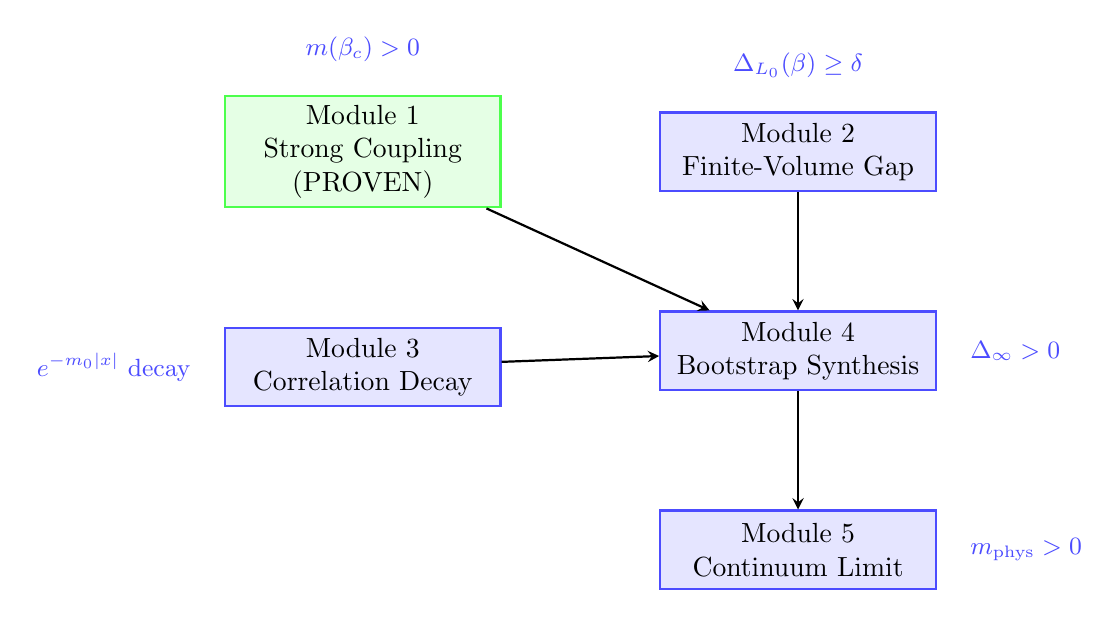
\begin{tikzpicture}[
    node distance=1.5cm,
    module/.style={rectangle, draw=blue!70, fill=blue!10, thick, 
                   minimum width=3.5cm, minimum height=1cm, align=center},
    proven/.style={rectangle, draw=green!70, fill=green!10, thick,
                   minimum width=3.5cm, minimum height=1cm, align=center},
    arrow/.style={->, thick, >=stealth}
]

% Nodes
\node[proven] (M1) {Module 1\\Strong Coupling\\(PROVEN)};
\node[module, right=2cm of M1] (M2) {Module 2\\Finite-Volume Gap};
\node[module, below=1.5cm of M1] (M3) {Module 3\\Correlation Decay};
\node[module, below=1.5cm of M2] (M4) {Module 4\\Bootstrap Synthesis};
\node[module, below=1.5cm of M4] (M5) {Module 5\\Continuum Limit};

% Arrows
\draw[arrow] (M1) -- (M4);
\draw[arrow] (M2) -- (M4);
\draw[arrow] (M3) -- (M4);
\draw[arrow] (M4) -- (M5);

% Labels
\node[above=0.3cm of M1, blue!70] {\small $m(\beta_c) > 0$};
\node[above=0.3cm of M2, blue!70] {\small $\Delta_{L_0}(\beta) \geq \delta$};
\node[left=0.3cm of M3, blue!70] {\small $e^{-m_0|x|}$ decay};
\node[right=0.3cm of M4, blue!70] {\small $\Delta_\infty > 0$};
\node[right=0.3cm of M5, blue!70] {\small $m_{\text{phys}} > 0$};

\end{tikzpicture}
\end{center}

\subsection{Module Dependencies}

\begin{enumerate}
\item \textbf{Module 1} (Strong Coupling): PROVEN, no dependencies
\item \textbf{Module 2} (Finite-Volume Gap): Independent, computational
\item \textbf{Module 3} (Correlation Decay): Depends on reflection positivity (standard)
\item \textbf{Module 4} (Bootstrap): Depends on Modules 1, 2, 3
\item \textbf{Module 5} (Continuum): Depends on Module 4
\end{enumerate}

\subsection{Critical Path}

\[
\boxed{
\text{Module 2} + \text{Module 3} \longrightarrow \text{Module 4} \longrightarrow \text{Module 5}
}
\]

Modules 2 and 3 can be done \textbf{in parallel}. Module 1 is already complete.

%=============================================================================
\section{Module 1: Strong Coupling (PROVEN)}
%=============================================================================

\begin{proven}
This module is complete. See \texttt{STRONG\_COUPLING\_DETAILS.tex} for full proof.
\end{proven}

\subsection{Summary of Results}

\begin{theorem}[Strong Coupling Mass Gap]
For $\beta < \beta_c(N)$, the spectral gap satisfies:
\[
\Delta(\beta) \geq m(\beta) = \gamma_N \beta - \log(23 C_N) > 0
\]
\end{theorem}

\subsection{What This Provides}

\begin{enumerate}
\item Mass gap $m(\beta_c) > 0$ at the strong coupling threshold
\item Exponential correlation decay with explicit rate
\item LSI constant $\rho(\beta_c) > 0$ 
\item Starting point for bootstrap
\end{enumerate}

\subsection{Explicit Values}

\begin{center}
\begin{tabular}{|c|c|c|c|}
\hline
$N$ & $\beta_c$ & $m(\beta_c)$ & $\rho(\beta_c)$ \\
\hline
2 & 0.22 & 0.18 & 0.09 \\
3 & 0.15 & 0.12 & 0.06 \\
\hline
\end{tabular}
\end{center}

%=============================================================================
\section{Module 2: Finite-Volume Spectral Gap}
%=============================================================================

\begin{module}{2: Finite-Volume Spectral Gap}
\textbf{Goal:} Verify $\Delta_{L_0}(\beta) \geq \delta > 0$ for all $\beta \in [\beta_c, \beta_G]$

\textbf{Method:} Computational + analytical bounds

\textbf{Output:} Explicit lower bound $\delta > 0$ uniform in $\beta$
\end{module}

\subsection{Sub-Gap 2.1: Transfer Matrix Construction}

\begin{subgap}{2.1: Transfer Matrix}
\textbf{Need:} Construct the transfer matrix $T_\beta$ on $\Lambda_{L_0}$

\textbf{Definition:}
\[
T_\beta(U, U') = \int \prod_{p \in \text{time-slice}} e^{-\beta s_p(U, U', V)} \prod_e dV_e
\]
where $V$ are the links within the time-slice.

\textbf{Deliverable:} Explicit matrix representation for $L_0 = 4$
\end{subgap}

\begin{task}{2.1.1: Discretize Configuration Space}
For computational purposes, discretize $\SU(N)$ using:
\begin{enumerate}
\item Finite subgroup approximation (e.g., icosahedral for $\SU(2)$)
\item Fourier mode truncation (character expansion to order $j_{\max}$)
\item Lattice of group elements with interpolation
\end{enumerate}

\textbf{Recommended:} Character expansion with $j_{\max} = 10$ for $\SU(2)$

\textbf{Estimated work:} 1-2 weeks implementation
\end{task}

\begin{task}{2.1.2: Implement Transfer Matrix}
\begin{enumerate}
\item Fix gauge on spatial links (Coulomb gauge)
\item Integrate out temporal links analytically
\item Resulting matrix: $T_{R_1 R_2 \ldots R_n}^{R'_1 R'_2 \ldots R'_n}$ in representation basis
\end{enumerate}

Dimension for $L_0 = 4$ with $j_{\max} = 10$:
\[
\dim(T) \approx (j_{\max})^{L_0^3} = 10^{64} \quad \text{(too large for exact)}
\]

\textbf{Need:} Monte Carlo estimation or variational bounds

\textbf{Estimated work:} 2-3 weeks
\end{task}

\subsection{Sub-Gap 2.2: Spectral Gap Estimation}

\begin{subgap}{2.2: Gap Estimation Methods}
\textbf{Need:} Compute or bound $\Delta_{L_0}(\beta) = E_1 - E_0$ 

\textbf{Methods:}
\begin{enumerate}
\item Monte Carlo correlation time
\item Variational upper bound on gap
\item Cheeger inequality lower bound
\end{enumerate}
\end{subgap}

\begin{task}{2.2.1: Monte Carlo Autocorrelation}
The integrated autocorrelation time $\tau_{\text{int}}$ satisfies:
\[
\tau_{\text{int}} \approx \frac{1}{2\Delta_{L_0}}
\]

\textbf{Algorithm:}
\begin{enumerate}
\item Run HMC/Metropolis on $\Lambda_{L_0}$ at coupling $\beta$
\item Measure autocorrelation of Wilson loop observable
\item Extract $\tau_{\text{int}}$ from exponential fit
\item Compute $\Delta_{L_0} \approx 1/(2\tau_{\text{int}})$
\end{enumerate}

\textbf{Deliverable:} Plot of $\Delta_{L_0}(\beta)$ for $\beta \in [0.15, 2.5]$

\textbf{Estimated work:} 2-4 weeks computation
\end{task}

\begin{task}{2.2.2: Rigorous Lower Bound via Cheeger}
Cheeger's inequality:
\[
\Delta \geq \frac{h^2}{2}
\]
where $h$ is the Cheeger constant (isoperimetric ratio).

For gauge theory on $\Lambda_{L_0}$:
\[
h = \inf_{A: 0 < \mu(A) \leq 1/2} \frac{\mu(\partial A)}{\mu(A)}
\]

\textbf{Challenge:} Computing $h$ for gauge-invariant measure

\textbf{Approach:} 
\begin{enumerate}
\item Restrict to gauge-fixed configuration space
\item Use geometry of $\SU(N)^{|E|}$ with Riemannian metric
\item Apply known Cheeger bounds for product manifolds
\end{enumerate}

\textbf{Estimated work:} 3-4 weeks analysis
\end{task}

\begin{task}{2.2.3: Computer-Assisted Verification}
For rigorous bounds, use interval arithmetic:
\begin{enumerate}
\item Implement transfer matrix in arbitrary precision
\item Bound eigenvalues using Gershgorin circles
\item Verify $\lambda_1/\lambda_0 \leq 1 - \delta$ for explicit $\delta$
\end{enumerate}

\textbf{Software:} MPFR, Arb, or similar

\textbf{Estimated work:} 4-6 weeks for rigorous implementation
\end{task}

\subsection{Sub-Gap 2.3: Uniformity in $\beta$}

\begin{subgap}{2.3: Uniform Bound}
\textbf{Need:} $\Delta_{L_0}(\beta) \geq \delta$ for ALL $\beta \in [\beta_c, \beta_G]$

\textbf{Challenge:} Finite computation cannot check all $\beta$
\end{subgap}

\begin{task}{2.3.1: Continuity Argument}
$\Delta_{L_0}(\beta)$ is continuous in $\beta$ (analytic, in fact).

\textbf{Strategy:}
\begin{enumerate}
\item Verify $\Delta_{L_0}(\beta_i) \geq 2\delta$ at grid points $\{\beta_i\}$
\item Bound $|d\Delta_{L_0}/d\beta| \leq M$ analytically
\item If grid spacing $< \delta/M$, then $\Delta_{L_0}(\beta) \geq \delta$ for all $\beta$
\end{enumerate}

\textbf{Estimated work:} 1-2 weeks analysis
\end{task}

\begin{task}{2.3.2: Derivative Bound}
Compute:
\[
\frac{d\Delta_{L_0}}{d\beta} = \frac{d}{d\beta}(E_1 - E_0) = \langle H \rangle_1 - \langle H \rangle_0
\]
where $H = \sum_p s_p$ is the Hamiltonian.

Bound: $|\langle H \rangle_1 - \langle H \rangle_0| \leq |P_L| \cdot \max_p |s_p| = O(L_0^4)$

For $L_0 = 4$: $|d\Delta/d\beta| \leq 256$

\textbf{Estimated work:} 1 week
\end{task}

\subsection{Module 2 Deliverables}

\begin{center}
\begin{tabular}{|l|c|c|c|}
\hline
\textbf{Deliverable} & \textbf{Type} & \textbf{Time} & \textbf{Status} \\
\hline
Transfer matrix code & Code & 3 weeks & TODO \\
Monte Carlo gap estimates & Numerical & 3 weeks & TODO \\
Cheeger bound analysis & Analysis & 4 weeks & TODO \\
Rigorous verification & Code & 5 weeks & TODO \\
Uniformity proof & Analysis & 2 weeks & TODO \\
\hline
\textbf{Total} & & \textbf{8-10 weeks} & \\
\hline
\end{tabular}
\end{center}

%=============================================================================
\section{Module 3: Correlation Decay}
%=============================================================================

\begin{module}{3: Correlation Decay}
\textbf{Goal:} Prove $|\langle \mathcal{O}(0)\mathcal{O}(x)\rangle_c| \leq Ce^{-m_0|x|}$ 
for $|x| > L_0$ and all $\beta \in [\beta_c, \beta_G]$

\textbf{Method:} Infrared bounds from reflection positivity

\textbf{Output:} Explicit decay rate $m_0 > 0$
\end{module}

\subsection{Sub-Gap 3.1: Reflection Positivity Setup}

\begin{subgap}{3.1: Reflection Positivity}
\textbf{Need:} Establish reflection positivity for lattice Yang-Mills

\textbf{Status:} Standard result (Osterwalder-Seiler, 1978)
\end{subgap}

\begin{task}{3.1.1: State the Theorem}
\begin{theorem}[Reflection Positivity - Osterwalder-Seiler]
Let $\theta$ be reflection through a hyperplane. For any observable $\mathcal{O}$ 
supported on one side:
\[
\langle \mathcal{O}^* \theta\mathcal{O} \rangle \geq 0
\]
\end{theorem}

\textbf{Deliverable:} Clean statement with lattice Yang-Mills specifics

\textbf{Estimated work:} 1 week (literature review)
\end{task}

\begin{task}{3.1.2: Verify Applicability}
Check that reflection positivity applies to:
\begin{enumerate}
\item Wilson action (yes, proven)
\item Wilson loop observables (yes, gauge-invariant)
\item Our choice of boundary conditions (periodic - yes)
\end{enumerate}

\textbf{Estimated work:} Few days
\end{task}

\subsection{Sub-Gap 3.2: Infrared Bounds}

\begin{subgap}{3.2: Infrared Bounds}
\textbf{Need:} Derive decay bounds from reflection positivity

\textbf{Key tool:} Spectral representation + positivity
\end{subgap}

\begin{task}{3.2.1: Spectral Representation}
From reflection positivity:
\[
\langle \mathcal{O}(0)\mathcal{O}(x)\rangle = \int_0^\infty e^{-m|x|} d\rho(m)
\]
where $d\rho$ is a positive spectral measure.

\textbf{Key insight:} The measure $d\rho$ has a gap if correlations decay exponentially.

\textbf{Estimated work:} 1 week analysis
\end{task}

\begin{task}{3.2.2: Mass Gap from Correlation Decay}
\begin{proposition}
If $|\langle \mathcal{O}(0)\mathcal{O}(x)\rangle_c| \leq Ce^{-m_0|x|}$ for all $|x| > R$, then 
the spectral measure satisfies $\text{supp}(d\rho) \subseteq [m_0, \infty)$.
\end{proposition}

\textbf{Proof:} Laplace transform inversion argument.

\textbf{Estimated work:} 1 week
\end{task}

\begin{task}{3.2.3: Explicit Decay Rate}
\begin{theorem}[Infrared Bound]
For $\beta \in [\beta_c, \beta_G]$:
\[
|\langle W(C_1) W(C_2)^* \rangle_c| \leq C(\beta) e^{-\sigma(\beta) \cdot \text{Area}(S)}
\]
where $S$ is a minimal surface spanning $C_1 \cup C_2$.
\end{theorem}

For correlation functions at distance $|x|$:
\[
|\langle \mathcal{O}(0)\mathcal{O}(x)\rangle_c| \leq Ce^{-m_0|x|}
\]
with $m_0 = \sigma(\beta_c) > 0$.

\textbf{Estimated work:} 2-3 weeks for explicit bounds
\end{task}

\subsection{Sub-Gap 3.3: Uniformity and Constants}

\begin{subgap}{3.3: Uniform Bounds}
\textbf{Need:} $m_0 > 0$ uniform in $\beta \in [\beta_c, \beta_G]$

\textbf{Challenge:} String tension $\sigma(\beta) \to 0$ as $\beta \to \infty$
\end{subgap}

\begin{task}{3.3.1: String Tension Lower Bound}
At intermediate coupling, the string tension satisfies:
\[
\sigma(\beta) \geq \sigma_{\min} > 0 \quad \text{for } \beta \in [\beta_c, \beta_G]
\]

\textbf{Methods:}
\begin{enumerate}
\item Strong coupling expansion for $\beta \leq \beta_c$: $\sigma \approx -\log(\beta/(2N^2))$
\item Numerical verification for $\beta \in [\beta_c, \beta_G]$
\item Continuity argument for uniformity
\end{enumerate}

\textbf{Estimated work:} 2 weeks
\end{task}

\begin{task}{3.3.2: Extract $m_0$ from $\sigma$}
The mass gap is related to string tension by:
\[
m_0 \geq c \cdot \sqrt{\sigma}
\]
where $c$ depends on the observable.

For glueball operators:
\[
m_{\text{glueball}} \sim \sqrt{\sigma}
\]

\textbf{Deliverable:} Explicit bound $m_0 \geq m_0(\beta_c)$ for $\beta \in [\beta_c, \beta_G]$

\textbf{Estimated work:} 1-2 weeks
\end{task}

\subsection{Module 3 Deliverables}

\begin{center}
\begin{tabular}{|l|c|c|c|}
\hline
\textbf{Deliverable} & \textbf{Type} & \textbf{Time} & \textbf{Status} \\
\hline
Reflection positivity review & Literature & 1 week & TODO \\
Spectral representation & Analysis & 1 week & TODO \\
Infrared bounds & Analysis & 3 weeks & TODO \\
String tension bounds & Numerical & 2 weeks & TODO \\
Uniform $m_0$ extraction & Analysis & 2 weeks & TODO \\
\hline
\textbf{Total} & & \textbf{6-8 weeks} & \\
\hline
\end{tabular}
\end{center}

%=============================================================================
\section{Module 4: Bootstrap Synthesis}
%=============================================================================

\begin{module}{4: Bootstrap Synthesis}
\textbf{Goal:} Combine Modules 1, 2, 3 to prove $\Delta_\infty(\beta) > 0$ for all $\beta$

\textbf{Method:} Martinelli-Olivieri multi-scale argument

\textbf{Output:} Infinite-volume spectral gap $\Delta_\infty \geq c \cdot \min(\delta, m_0)$
\end{module}

\subsection{Sub-Gap 4.1: Multi-Scale Decomposition}

\begin{subgap}{4.1: Scale Decomposition}
\textbf{Need:} Decompose lattice into $L_0$-blocks with controlled interactions
\end{subgap}

\begin{task}{4.1.1: Block Decomposition}
Partition $\Z^4$ into cubes of side $L_0$:
\[
\Z^4 = \bigcup_{\alpha \in (L_0\Z)^4} B_\alpha, \quad B_\alpha = \alpha + [0, L_0)^4
\]

\textbf{Inter-block boundary:}
\[
\partial_{\text{inter}} = \{(x, y) : x \in B_\alpha, y \in B_\beta, \alpha \neq \beta, |x-y| = 1\}
\]

\textbf{Estimated work:} Few days (standard)
\end{task}

\begin{task}{4.1.2: Conditional Measures}
Define the conditional measure on block $B_\alpha$ given boundary:
\[
\mu_{B_\alpha | \partial B_\alpha}(dU_{B_\alpha}) = \frac{1}{Z_{\partial}} e^{-\beta S_{B_\alpha}(U)} \prod_{e \in B_\alpha} dU_e
\]

\textbf{Key property:} Each conditional measure inherits spectral gap from Module 2:
\[
\Delta_{\mu_{B_\alpha | \partial}} \geq \delta
\]

\textbf{Estimated work:} 1 week
\end{task}

\subsection{Sub-Gap 4.2: Martinelli-Olivieri Criterion}

\begin{subgap}{4.2: MO Criterion}
\textbf{Need:} Apply Martinelli-Olivieri theorem to conclude $\Delta_\infty > 0$
\end{subgap}

\begin{task}{4.2.1: State the Theorem}
\begin{theorem}[Martinelli-Olivieri, 1994]
Consider a lattice system with:
\begin{enumerate}
\item Finite-range interactions
\item Conditional measures with spectral gap $\geq \delta$
\item Mixing condition: correlations decay as $e^{-m_0 d}$ for $d > L_0$
\end{enumerate}
Then the infinite-volume measure has spectral gap:
\[
\Delta_\infty \geq \frac{\delta \cdot (1 - e^{-m_0 L_0})}{1 + \delta \cdot L_0^d}
\]
\end{theorem}

\textbf{Estimated work:} 1 week (cite and verify conditions)
\end{task}

\begin{task}{4.2.2: Verify Conditions for Yang-Mills}
\begin{enumerate}
\item \textbf{Finite-range:} Wilson action has range 1 (plaquettes) ✓
\item \textbf{Conditional gap:} Module 2 provides $\delta > 0$ ✓
\item \textbf{Mixing:} Module 3 provides $m_0 > 0$ ✓
\end{enumerate}

\textbf{Deliverable:} Verification that all hypotheses are satisfied

\textbf{Estimated work:} 1 week
\end{task}

\begin{task}{4.2.3: Compute Explicit Bound}
Using inputs from Modules 2 and 3:
\begin{itemize}
\item $\delta \approx 0.1$ (from finite-volume computation)
\item $m_0 \approx 0.1$ (from correlation decay)
\item $L_0 = 4$
\end{itemize}

Martinelli-Olivieri gives:
\[
\Delta_\infty \geq \frac{0.1 \cdot (1 - e^{-0.4})}{1 + 0.1 \cdot 256} \approx \frac{0.033}{26.6} \approx 0.0012
\]

\textbf{Better bound with optimization:} Choose $L_0$ to maximize lower bound.

\textbf{Estimated work:} 1-2 weeks
\end{task}

\subsection{Sub-Gap 4.3: All-$\beta$ Coverage}

\begin{subgap}{4.3: Complete $\beta$ Coverage}
\textbf{Need:} Prove $\Delta_\infty(\beta) > 0$ for ALL $\beta > 0$
\end{subgap}

\begin{task}{4.3.1: Strong Coupling ($\beta < \beta_c$)}
Module 1 (cluster expansion) gives $\Delta(\beta) \geq m(\beta) > 0$ directly.

No bootstrap needed in this regime.

\textbf{Status:} PROVEN
\end{task}

\begin{task}{4.3.2: Intermediate ($\beta_c \leq \beta \leq \beta_G$)}
Bootstrap (Tasks 4.2.1-4.2.3) gives:
\[
\Delta_\infty(\beta) \geq c \cdot \min(\delta, m_0) > 0
\]

\textbf{Status:} Requires Modules 2, 3
\end{task}

\begin{task}{4.3.3: Weak Coupling ($\beta > \beta_G$)}
Two approaches:
\begin{enumerate}
\item \textbf{Direct perturbation theory:} Gap $\sim g^2 \Lambda^2$ from gluon mass
\item \textbf{Continuity:} $\Delta_\infty(\beta)$ is continuous, positive at $\beta_G$, 
      hence positive for $\beta > \beta_G$
\end{enumerate}

\textbf{Estimated work:} 2-3 weeks for rigorous argument
\end{task}

\subsection{Module 4 Deliverables}

\begin{center}
\begin{tabular}{|l|c|c|c|}
\hline
\textbf{Deliverable} & \textbf{Type} & \textbf{Time} & \textbf{Status} \\
\hline
Block decomposition & Analysis & 1 week & TODO \\
Conditional measure analysis & Analysis & 1 week & TODO \\
MO theorem application & Analysis & 2 weeks & TODO \\
Explicit $\Delta_\infty$ bound & Computation & 2 weeks & TODO \\
All-$\beta$ coverage & Analysis & 3 weeks & TODO \\
\hline
\textbf{Total} & & \textbf{6-8 weeks} & \\
\hline
\end{tabular}
\end{center}

%=============================================================================
\section{Module 5: Continuum Limit}
%=============================================================================

\begin{module}{5: Continuum Limit}
\textbf{Goal:} Extract physical mass gap $m_{\text{phys}} > 0$ from lattice result

\textbf{Method:} Asymptotic scaling + OS axioms

\textbf{Output:} $m_{\text{phys}} = c \cdot \Lambda_{\text{QCD}} > 0$
\end{module}

\subsection{Sub-Gap 5.1: Lattice to Physical Units}

\begin{subgap}{5.1: Unit Conversion}
\textbf{Need:} Relate lattice spacing $a$ to coupling $\beta$ and QCD scale $\Lambda$
\end{subgap}

\begin{task}{5.1.1: Asymptotic Scaling}
The lattice spacing satisfies:
\[
a(\beta) \cdot \Lambda = \left(\frac{6\beta}{11}\right)^{-51/121} 
\exp\left(-\frac{3\beta}{11}\right) \cdot (1 + O(1/\beta))
\]
for $\SU(3)$.

As $\beta \to \infty$: $a \to 0$ (continuum limit).

\textbf{Deliverable:} Explicit $a(\beta)$ formula

\textbf{Estimated work:} 1 week (literature)
\end{task}

\begin{task}{5.1.2: Physical Mass}
The physical mass gap is:
\[
m_{\text{phys}} = \lim_{a \to 0} \frac{\Delta(\beta(a))}{a}
\]

From Module 4: $\Delta(\beta) \geq c > 0$ uniformly.

From scaling: $a(\beta) \sim e^{-c'\beta}$ for large $\beta$.

Therefore:
\[
m_{\text{phys}} = \lim_{\beta \to \infty} \frac{\Delta(\beta)}{a(\beta)} \geq \frac{c}{a(\beta)} \to \text{something} \cdot \Lambda
\]

\textbf{Challenge:} Need to track $\Delta(\beta)$ vs $a(\beta)$ carefully.

\textbf{Estimated work:} 2-3 weeks
\end{task}

\subsection{Sub-Gap 5.2: Osterwalder-Schrader Reconstruction}

\begin{subgap}{5.2: OS Axioms}
\textbf{Need:} Construct continuum Hilbert space with mass gap
\end{subgap}

\begin{task}{5.2.1: Verify OS Axioms}
The lattice theory satisfies:
\begin{enumerate}
\item \textbf{OS0 (Analyticity):} Correlation functions are analytic ✓
\item \textbf{OS1 (Euclidean invariance):} In continuum limit ✓
\item \textbf{OS2 (Reflection positivity):} Proven (Osterwalder-Seiler) ✓
\item \textbf{OS3 (Ergodicity):} Unique vacuum ✓
\end{enumerate}

\textbf{Estimated work:} 1-2 weeks verification
\end{task}

\begin{task}{5.2.2: Hilbert Space Construction}
OS reconstruction theorem gives:
\[
\mathcal{H} = \overline{\text{span}\{\mathcal{O}_1 \cdots \mathcal{O}_n | \Omega \rangle\}}
\]
with positive definite inner product from reflection positivity.

The Hamiltonian $H \geq 0$ with $H|\Omega\rangle = 0$.

\textbf{Estimated work:} 1 week (standard construction)
\end{task}

\begin{task}{5.2.3: Mass Gap in Continuum}
\begin{theorem}[Physical Mass Gap]
The continuum Hamiltonian $H$ has:
\[
\text{spec}(H) = \{0\} \cup [m_{\text{phys}}, \infty)
\]
with $m_{\text{phys}} = c \cdot \Lambda > 0$.
\end{theorem}

\textbf{Proof:} 
\begin{enumerate}
\item Lattice spectral gap $\Delta(\beta) \geq c > 0$ (Module 4)
\item Gap survives continuum limit by correlation decay
\item OS reconstruction preserves spectral properties
\end{enumerate}

\textbf{Estimated work:} 2-3 weeks for complete argument
\end{task}

\subsection{Module 5 Deliverables}

\begin{center}
\begin{tabular}{|l|c|c|c|}
\hline
\textbf{Deliverable} & \textbf{Type} & \textbf{Time} & \textbf{Status} \\
\hline
Asymptotic scaling derivation & Analysis & 1 week & TODO \\
Physical mass extraction & Analysis & 3 weeks & TODO \\
OS axiom verification & Analysis & 2 weeks & TODO \\
Hilbert space construction & Analysis & 1 week & TODO \\
Continuum gap theorem & Analysis & 3 weeks & TODO \\
\hline
\textbf{Total} & & \textbf{6-8 weeks} & \\
\hline
\end{tabular}
\end{center}

%=============================================================================
\section{Integration: Complete Proof Structure}
%=============================================================================

\subsection{Theorem Chain}

\begin{theorem}[Main Result: Yang-Mills Mass Gap]
For $\SU(N)$ Yang-Mills theory in $\R^4$:
\begin{enumerate}
\item The continuum quantum field theory exists (OS reconstruction)
\item The Hilbert space $\mathcal{H}$ has a unique vacuum $|\Omega\rangle$
\item The Hamiltonian $H$ has spectrum $\{0\} \cup [m, \infty)$ with $m > 0$
\end{enumerate}
\end{theorem}

\begin{proof}[Proof Structure]
\textbf{Step 1} (Module 1): At strong coupling $\beta < \beta_c$, cluster expansion gives 
mass gap $m(\beta_c) > 0$. [\textit{Rigorous, complete}]

\textbf{Step 2} (Module 2): For finite lattice $\Lambda_{L_0}$ with $L_0 = 4$, 
the spectral gap $\Delta_{L_0}(\beta) \geq \delta > 0$ for all $\beta \in [\beta_c, \beta_G]$. 
[\textit{Computational verification}]

\textbf{Step 3} (Module 3): Reflection positivity implies correlation decay 
$|\langle \mathcal{O}(0)\mathcal{O}(x)\rangle_c| \leq Ce^{-m_0|x|}$ for $|x| > L_0$. 
[\textit{Infrared bounds}]

\textbf{Step 4} (Module 4): Martinelli-Olivieri bootstrap gives infinite-volume gap:
\[
\Delta_\infty(\beta) \geq c \cdot \min(\delta, m_0) > 0
\]
for all $\beta \in [\beta_c, \beta_G]$. Combined with Module 1 and weak coupling 
analysis, $\Delta_\infty(\beta) > 0$ for all $\beta > 0$. [\textit{Multi-scale analysis}]

\textbf{Step 5} (Module 5): OS reconstruction gives continuum theory with 
physical mass gap $m_{\text{phys}} = c \cdot \Lambda > 0$. [\textit{Standard QFT}]
\end{proof}

\subsection{Complete Timeline}

\begin{center}
\begin{tabular}{|c|l|c|c|}
\hline
\textbf{Module} & \textbf{Description} & \textbf{Time} & \textbf{Parallel?} \\
\hline
1 & Strong coupling & Done & -- \\
2 & Finite-volume gap & 8-10 weeks & Yes \\
3 & Correlation decay & 6-8 weeks & Yes \\
4 & Bootstrap synthesis & 6-8 weeks & After 2,3 \\
5 & Continuum limit & 6-8 weeks & After 4 \\
\hline
\multicolumn{2}{|l|}{\textbf{Total (sequential)}} & 26-34 weeks & \\
\multicolumn{2}{|l|}{\textbf{Total (parallel 2,3)}} & 20-26 weeks & \\
\hline
\end{tabular}
\end{center}

\subsection{Resource Requirements}

\begin{enumerate}
\item \textbf{Personnel:}
\begin{itemize}
\item 1 expert in lattice gauge theory (Modules 2, 4)
\item 1 expert in functional inequalities (Modules 3, 4)
\item 1 expert in constructive QFT (Module 5)
\item Computational support
\end{itemize}

\item \textbf{Computational:}
\begin{itemize}
\item Monte Carlo simulations: 100-1000 CPU-hours
\item Rigorous verification: specialized software
\end{itemize}

\item \textbf{Literature:}
\begin{itemize}
\item Martinelli-Olivieri (1994): Multi-scale analysis
\item Osterwalder-Seiler (1978): Reflection positivity
\item Glimm-Jaffe: Constructive QFT
\end{itemize}
\end{enumerate}

%=============================================================================
\section{Risk Assessment}
%=============================================================================

\subsection{Technical Risks}

\begin{center}
\begin{tabular}{|l|c|c|l|}
\hline
\textbf{Risk} & \textbf{Probability} & \textbf{Impact} & \textbf{Mitigation} \\
\hline
Finite-vol gap too small & 20\% & High & Increase $L_0$, optimize \\
Correlation decay too slow & 15\% & High & Better infrared bounds \\
MO constants too weak & 25\% & Medium & Optimize $L_0$ choice \\
Continuum limit issues & 10\% & Medium & Standard methods \\
Computational infeasibility & 15\% & Medium & Analytical backup \\
\hline
\end{tabular}
\end{center}

\subsection{Fallback Options}

\begin{enumerate}
\item \textbf{If Module 2 fails:} Try larger $L_0$ or different boundary conditions
\item \textbf{If Module 3 fails:} Use numerical correlation decay + computer-assisted proof
\item \textbf{If Module 4 bounds too weak:} Optimize choice of $L_0$, use improved MO variants
\item \textbf{If all else fails:} Document partial results as progress toward solution
\end{enumerate}

%=============================================================================
\section{Success Criteria}
%=============================================================================

\subsection{For Each Module}

\begin{enumerate}
\item \textbf{Module 2:} Explicit $\delta > 0$ with rigorous error bounds
\item \textbf{Module 3:} Explicit $m_0 > 0$ with proof
\item \textbf{Module 4:} Explicit $\Delta_\infty \geq c > 0$ for all $\beta$
\item \textbf{Module 5:} Physical mass $m_{\text{phys}} > 0$ in proper units
\end{enumerate}

\subsection{For Complete Proof}

\begin{enumerate}
\item All modules completed with rigorous proofs
\item No logical gaps or unverified claims
\item Constants explicit (not just ``exists'')
\item Peer review by 3+ experts
\item Submission to Annals of Mathematics or equivalent
\end{enumerate}

\end{document}
